\documentclass[border=8pt]{standalone}
\usepackage[utf8]{inputenc}
\usepackage[T1]{fontenc}
\usepackage{amsmath,amssymb}
\usepackage{tikz}
\usetikzlibrary{shapes.geometric,arrows.meta,positioning,fit,backgrounds,calc}

\begin{document}
\hyphenpenalty=10000\exhyphenpenalty=10000
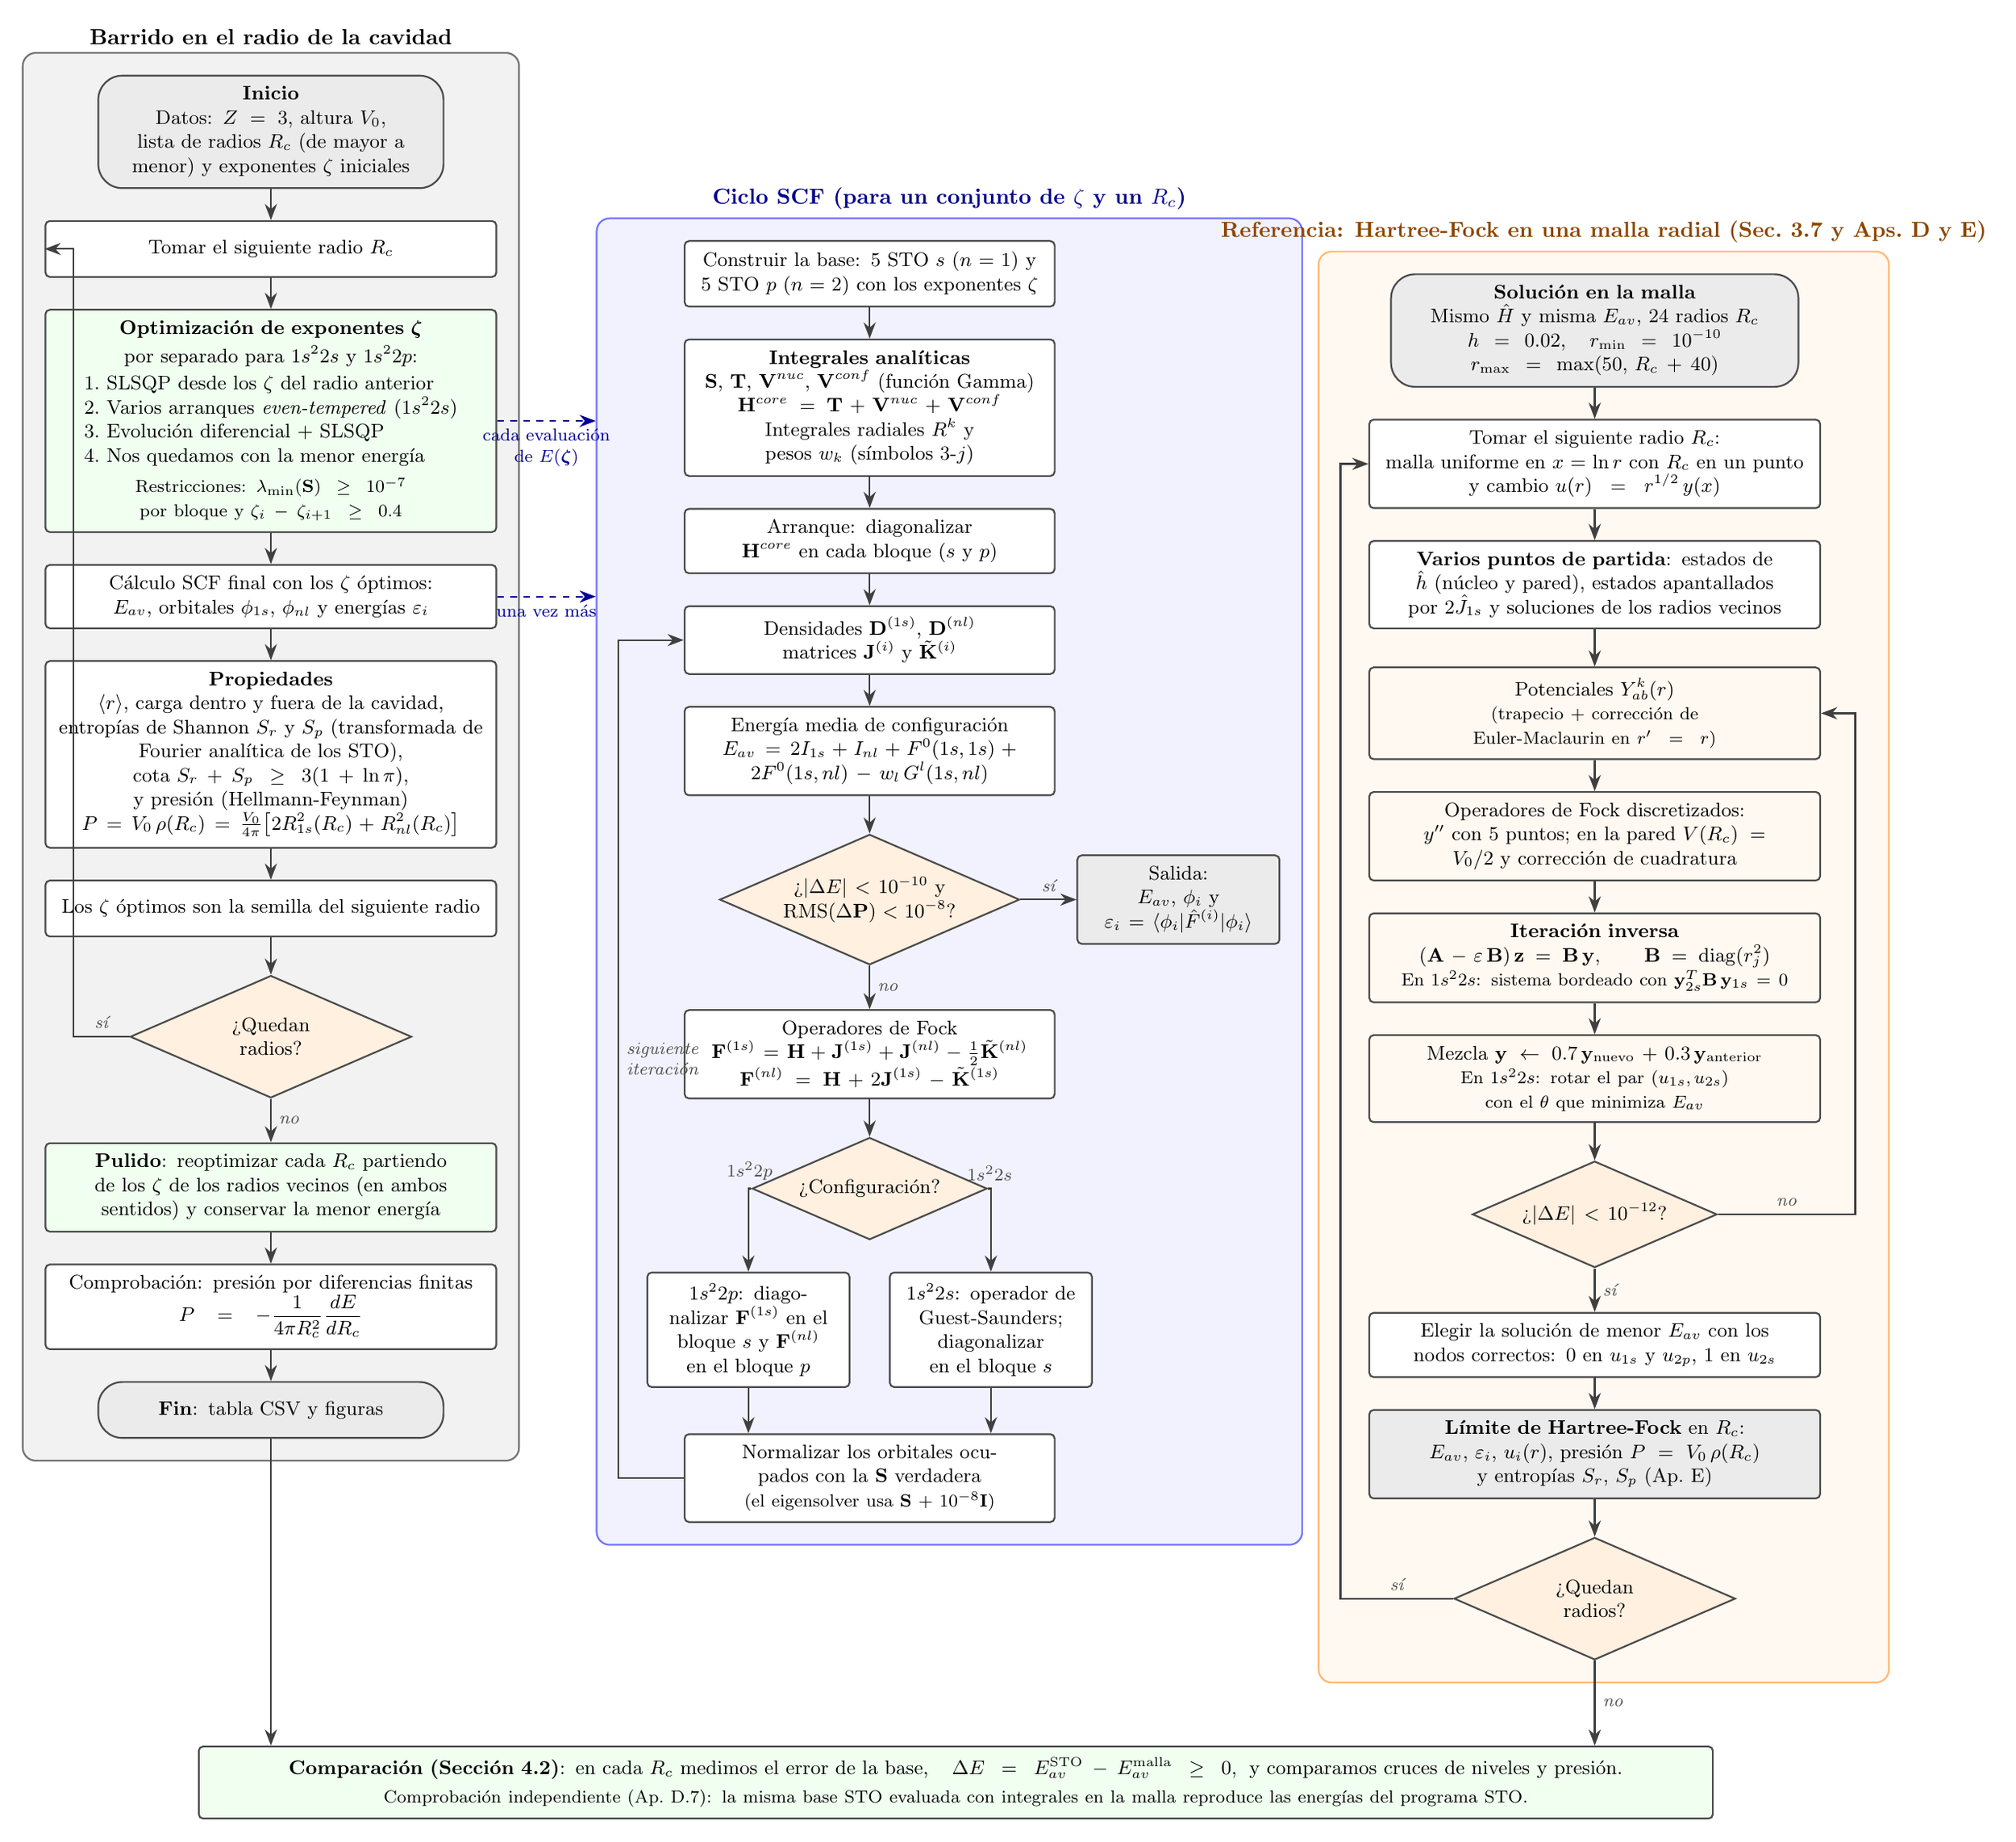
\begin{tikzpicture}[
    font=\small,
    node distance=5mm and 10mm,
    >={Stealth[length=2.6mm]},
    flecha/.style={->,thick,draw=black!75},
    llamada/.style={->,thick,dashed,draw=blue!60!black},
    proceso/.style={rectangle,rounded corners=2pt,draw=black!70,fill=white,thick,
                    text width=6.9cm,align=center,inner sep=5pt,minimum height=9mm},
    proc2/.style={proceso,text width=5.6cm},
    inicio/.style={rectangle,rounded corners=11pt,draw=black!70,fill=black!8,thick,
                   text width=5.2cm,align=center,inner sep=5pt,minimum height=9mm},
    decision/.style={diamond,aspect=2.3,draw=black!70,fill=orange!12,thick,
                     align=center,inner sep=1pt,text width=2.9cm},
    etiqueta/.style={font=\footnotesize\itshape,text=black!70},
    marco/.style={rectangle,rounded corners=6pt,draw=#1!55,fill=#1!5,thick,inner sep=8pt},
    titulo/.style={font=\bfseries\normalsize,text=#1!55!black},
]

% ===================== COLUMNA IZQUIERDA: barrido en R_c =====================
\node[inicio] (ini) {\textbf{Inicio}\\ Datos: $Z=3$, altura $V_0$, lista de radios $R_c$ (de mayor a menor) y exponentes $\zeta$ iniciales};

\node[proceso, below=of ini] (radio) {Tomar el siguiente radio $R_c$};

\node[proceso, below=of radio, fill=green!6] (opt) {\textbf{Optimización de exponentes} $\boldsymbol{\zeta}$\\[2pt]
  por separado para $1s^2 2s$ y $1s^2 2p$:\\[2pt]
  \begin{tabular}{@{}l@{}}
  1.\ SLSQP desde los $\zeta$ del radio anterior\\
  2.\ Varios arranques \emph{even-tempered} ($1s^2 2s$)\\
  3.\ Evolución diferencial $+$ SLSQP\\
  4.\ Nos quedamos con la menor energía
  \end{tabular}\\[3pt]
  {\footnotesize Restricciones: $\lambda_{\min}(\mathbf{S}) \ge 10^{-7}$ por bloque y $\zeta_i - \zeta_{i+1} \ge 0.4$}};

\node[proceso, below=of opt] (final) {Cálculo SCF final con los $\zeta$ óptimos:\\ $E_{av}$, orbitales $\phi_{1s}$, $\phi_{nl}$ y energías $\varepsilon_i$};

\node[proceso, below=of final] (prop) {\textbf{Propiedades}\\
  $\langle r\rangle$, carga dentro y fuera de la cavidad,\\
  entropías de Shannon $S_r$ y $S_p$ (transformada de\\
  Fourier analítica de los STO), cota $S_r + S_p \ge 3(1+\ln\pi)$,\\
  y presión (Hellmann-Feynman)\\
  $P = V_0\,\rho(R_c) = \tfrac{V_0}{4\pi}\big[2R_{1s}^2(R_c) + R_{nl}^2(R_c)\big]$};

\node[proceso, below=of prop] (semilla) {Los $\zeta$ óptimos son la semilla del siguiente radio};

\node[decision, below=6mm of semilla] (mas) {¿Quedan\\ radios?};

\node[proceso, below=7mm of mas, fill=green!6] (pulir) {\textbf{Pulido}: reoptimizar cada $R_c$ partiendo de los $\zeta$ de los radios vecinos (en ambos sentidos) y conservar la menor energía};

\node[proceso, below=of pulir] (fd) {Comprobación: presión por diferencias finitas\\ $P = -\dfrac{1}{4\pi R_c^2}\dfrac{dE}{dR_c}$};

\node[inicio, below=of fd] (fin) {\textbf{Fin}: tabla CSV y figuras};

\draw[flecha] (ini) -- (radio);
\draw[flecha] (radio) -- (opt);
\draw[flecha] (opt) -- (final);
\draw[flecha] (final) -- (prop);
\draw[flecha] (prop) -- (semilla);
\draw[flecha] (semilla) -- (mas);
\draw[flecha] (mas) -- node[right,etiqueta]{no} (pulir);
\draw[flecha] (mas.west) -- node[above,etiqueta]{sí} ++(-0.9,0) |- (radio.west);
\draw[flecha] (pulir) -- (fd);
\draw[flecha] (fd) -- (fin);

% ===================== COLUMNA DERECHA: ciclo SCF =====================
\node[proc2, right=30mm of radio, yshift=-4mm] (base) {Construir la base: 5 STO $s$ ($n=1$) y 5 STO $p$ ($n=2$) con los exponentes $\zeta$};

\node[proc2, below=of base] (ints) {\textbf{Integrales analíticas}\\
  $\mathbf{S}$, $\mathbf{T}$, $\mathbf{V}^{nuc}$, $\mathbf{V}^{conf}$ (función Gamma)\\
  $\mathbf{H}^{core} = \mathbf{T} + \mathbf{V}^{nuc} + \mathbf{V}^{conf}$\\
  Integrales radiales $R^k$ y pesos $w_k$ (símbolos 3-$j$)};

\node[proc2, below=of ints] (arranque) {Arranque: diagonalizar $\mathbf{H}^{core}$ en cada bloque ($s$ y $p$)};

\node[proc2, below=of arranque] (dens) {Densidades $\mathbf{D}^{(1s)}$, $\mathbf{D}^{(nl)}$\\ matrices $\mathbf{J}^{(i)}$ y $\tilde{\mathbf{K}}^{(i)}$};

\node[proc2, below=of dens] (eav) {Energía media de configuración\\
  $E_{av} = 2I_{1s} + I_{nl} + F^0(1s,1s) + 2F^0(1s,nl) - w_l\, G^l(1s,nl)$};

\node[decision, below=6mm of eav] (conv) {¿$|\Delta E| < 10^{-10}$ y\\ $\mathrm{RMS}(\Delta\mathbf{P}) < 10^{-8}$?};

\node[proc2, below=7mm of conv] (fock) {Operadores de Fock\\
  $\mathbf{F}^{(1s)} = \mathbf{H} + \mathbf{J}^{(1s)} + \mathbf{J}^{(nl)} - \tfrac12\tilde{\mathbf{K}}^{(nl)}$\\
  $\mathbf{F}^{(nl)} = \mathbf{H} + 2\mathbf{J}^{(1s)} - \tilde{\mathbf{K}}^{(1s)}$};

\node[decision, below=6mm of fock] (cfg) {¿Configuración?};

\node[proc2, text width=2.9cm, anchor=north] (d2p) at ($(cfg.south)+(-1.95,-0.5)$) {\textbf{$1s^2 2p$}: diagonalizar $\mathbf{F}^{(1s)}$ en el bloque $s$ y $\mathbf{F}^{(nl)}$ en el bloque $p$};
\node[proc2, text width=2.9cm, anchor=north] (d2s) at ($(cfg.south)+(1.95,-0.5)$) {\textbf{$1s^2 2s$}: operador de Guest-Saunders; diagonalizar en el bloque $s$};

\node[proc2, anchor=north] (renorm) at ($(cfg.south)+(0,-3.1)$) {Normalizar los orbitales ocupados con la $\mathbf{S}$ verdadera\\ {\footnotesize (el eigensolver usa $\mathbf{S} + 10^{-8}\mathbf{I}$)}};

\node[proc2, right=9mm of conv, text width=2.9cm, fill=black!8] (sal) {Salida:\\ $E_{av}$, $\phi_i$ y\\ $\varepsilon_i = \langle\phi_i|\hat F^{(i)}|\phi_i\rangle$};

\draw[flecha] (base) -- (ints);
\draw[flecha] (ints) -- (arranque);
\draw[flecha] (arranque) -- (dens);
\draw[flecha] (dens) -- (eav);
\draw[flecha] (eav) -- (conv);
\draw[flecha] (conv) -- node[above,etiqueta]{sí} (sal);
\draw[flecha] (conv) -- node[right,etiqueta]{no} (fock);
\draw[flecha] (fock) -- (cfg);
\draw[flecha] (cfg.west) -| node[pos=0.3,above,etiqueta]{$1s^2 2p$} (d2p.north);
\draw[flecha] (cfg.east) -| node[pos=0.3,above,etiqueta]{$1s^2 2s$} (d2s.north);
\draw[flecha] (d2p.south) -- (d2p.south |- renorm.north);
\draw[flecha] (d2s.south) -- (d2s.south |- renorm.north);
\coordinate (xr) at ($(d2p.west)+(-0.45,0)$);
\draw[flecha] (renorm.west) -- (renorm.west -| xr) |- node[pos=0.25,right,etiqueta,align=left]{siguiente\\ iteración} (dens.west);

% ===================== MARCOS =====================
\begin{scope}[on background layer]
  \node[marco=black, fit=(ini)(radio)(opt)(final)(prop)(semilla)(mas)(pulir)(fd)(fin), inner sep=10pt, label={[titulo=black]above:Barrido en el radio de la cavidad}] (A) {};
  \node[marco=blue, fit=(base)(ints)(arranque)(dens)(eav)(conv)(fock)(cfg)(d2p)(d2s)(renorm)(sal)(xr), inner xsep=10pt, inner ysep=10pt, label={[titulo=blue]above:Ciclo SCF (para un conjunto de $\zeta$ y un $R_c$)}] (B) {};
\end{scope}

% Llamadas al SCF
\draw[llamada] (opt.east) -- node[below,font=\footnotesize,text=blue!60!black,align=center]{cada evaluación\\ de $E(\boldsymbol\zeta)$} (opt.east -| B.west);
\draw[llamada] (final.east) -- node[below,font=\footnotesize,text=blue!60!black]{una vez más} (final.east -| B.west);

% ===================== COLUMNA DERECHA: malla radial (Apéndice D) =====================
\node[inicio, anchor=north west, text width=6.2cm] (g0) at ($(B.north east)+(1.4,-0.9)$) {\textbf{Solución en la malla}\\ Mismo $\hat H$ y misma $E_{av}$, 24 radios $R_c$\\ $h = 0.02,\quad r_{\min} = 10^{-10}$\\ $r_{\max} = \max(50,\,R_c+40)$};

\node[proceso, below=of g0] (g1) {Tomar el siguiente radio $R_c$:\\ malla uniforme en $x = \ln r$ con $R_c$ en un punto\\ y cambio $u(r) = r^{1/2}\,y(x)$};

\node[proceso, below=of g1] (g2) {\textbf{Varios puntos de partida}: estados de $\hat h$ (núcleo y pared), estados apantallados por $2\hat J_{1s}$ y soluciones de los radios vecinos};

\node[proceso, below=6mm of g2, fill=orange!5] (g3) {Potenciales $Y^k_{ab}(r)$\\ {\footnotesize (trapecio $+$ corrección de Euler-Maclaurin en $r' = r$)}};

\node[proceso, below=of g3, fill=orange!5] (g4) {Operadores de Fock discretizados:\\ $y''$ con 5 puntos; en la pared $V(R_c) = V_0/2$ y corrección de cuadratura};

\node[proceso, below=of g4, fill=orange!5] (g5) {\textbf{Iteración inversa}\\ $(\mathbf A - \varepsilon\,\mathbf B)\,\mathbf z = \mathbf B\,\mathbf y, \qquad \mathbf B = \mathrm{diag}(r_j^2)$\\ {\footnotesize En $1s^2 2s$: sistema bordeado con $\mathbf y_{2s}^{T}\mathbf B\,\mathbf y_{1s} = 0$}};

\node[proceso, below=of g5, fill=orange!5] (g6) {Mezcla $\mathbf y \leftarrow 0.7\,\mathbf y_{\mathrm{nuevo}} + 0.3\,\mathbf y_{\mathrm{anterior}}$\\ {\footnotesize En $1s^2 2s$: rotar el par $(u_{1s},u_{2s})$ con el $\theta$ que minimiza $E_{av}$}};

\node[decision, below=6mm of g6] (g7) {¿$|\Delta E| < 10^{-12}$?};

\node[proceso, below=7mm of g7] (g8) {Elegir la solución de menor $E_{av}$ con los nodos correctos: 0 en $u_{1s}$ y $u_{2p}$, 1 en $u_{2s}$};

\node[proceso, below=of g8, fill=black!8] (g9) {\textbf{Límite de Hartree-Fock} en $R_c$:\\ $E_{av}$, $\varepsilon_i$, $u_i(r)$, presión $P = V_0\,\rho(R_c)$\\ y entropías $S_r$, $S_p$ (Ap.~E)};

\node[decision, below=6mm of g9] (g10) {¿Quedan\\ radios?};

\draw[flecha] (g0) -- (g1);
\draw[flecha] (g1) -- (g2);
\draw[flecha] (g2) -- (g3);
\draw[flecha] (g3) -- (g4);
\draw[flecha] (g4) -- (g5);
\draw[flecha] (g5) -- (g6);
\draw[flecha] (g6) -- (g7);
\draw[flecha] (g7) -- node[right,etiqueta]{sí} (g8);
\coordinate (xg) at ($(g3.east)+(0.55,0)$);
\draw[flecha] (g7.east) -- (g7.east -| xg) node[pos=0.5,above,etiqueta]{no} |- (g3.east);
\draw[flecha] (g8) -- (g9);
\draw[flecha] (g9) -- (g10);
\coordinate (xg2) at ($(g1.west)+(-0.45,0)$);
\draw[flecha] (g10.west) -- (g10.west -| xg2) node[pos=0.5,above,etiqueta]{sí} |- (g1.west);

\begin{scope}[on background layer]
  \node[rectangle,rounded corners=4pt,draw=orange!60,dashed,thick,fit=(g3)(g4)(g5)(g6)(g7)(xg), inner sep=5pt, label={[font=\footnotesize\bfseries,text=orange!60!black,anchor=south east]north east:ciclo SCF en la malla}] (GS) {};
  \node[marco=orange, fit=(g0)(g1)(g2)(GS)(g8)(g9)(g10)(xg2), inner sep=10pt, label={[titulo=orange]above:Referencia: Hartree-Fock en una malla radial (Sec.~3.7 y Aps.~D y E)}] (C) {};
\end{scope}

% ===================== COMPARACIÓN =====================
\coordinate (cx) at ($(A.west)!0.5!(C.east)$);
\node[proceso, text width=24cm, fill=green!6, anchor=north] (comp) at ($(cx |- C.south)+(0,-1.0)$) {\textbf{Comparación (Sección 4.2)}: en cada $R_c$ medimos el error de la base, $\;\Delta E = E_{av}^{\mathrm{STO}} - E_{av}^{\mathrm{malla}} \ge 0$, \;y comparamos cruces de niveles y presión.\\[2pt]
{\footnotesize Comprobación independiente (Ap.~D.7): la misma base STO evaluada con integrales en la malla reproduce las energías del programa STO.}};

\draw[flecha] (fin.south) -- (fin.south |- comp.north);
\draw[flecha] (g10.south) -- node[right,etiqueta]{no} (g10.south |- comp.north);

\end{tikzpicture}
\end{document}
